\chapter{Underground Seismic Noise}

\section{Seismic Noise}
\subsection{Overview}
Seismic noise cause two main problems to the terrestrial gravitational-wave detectors.

First, the noise limits the sensitivity of the detectors in lower frequency especially below 10 $\mathrm{Hz}$. As mentioned in \cref{sec:13}, the laser interferometric detector recieves the gravitational-wave signal in the DARM signal, which is the length difference of the X arm and the Y arm. The noise disturb these arm length. Therefore, in order to detect the signal in lower frequencies, we have developed the vibration isolation system reducing the seismic noise \cite{takamori2002low},\cite{sekiguchi2016astudy},\cite{Okutomi2019development}.

Second, the noise decrease the duty cycle of the detectors. Realistically, it is difficult to reduce the seismic noise below 0.1 $\mathrm{Hz}$. This difficulty means that the motions not adequately isolated disturb the detector which only can work within the limited range. 

Under ground can resolve these problems. Places under the ground are more quiet than these on the surface of the ground \cite{carter1991high}. Especially, the seismic noise of the underground above 1 $\mathrm{Hz}$ is effectivly reduced than the noise of the surface \cite{lcgt2009lcgt}. 世界で初めて地下に建設した20mの重力波望遠鏡LISMはその安定性の高さを示した\cite{sato2004ultrastable}。

しかしながら、長期線の検出器においては、後者のDuty Cycleの向上はさほど望めない。なぜならば、詳細は\cref{sec:32}で述べるが、基線長が長くなると地面振動は基線長伸縮に現れやすくなるためである。例えば、基線長が短いと地面振動は基線全体を動かす。つまり基線長伸縮に現れにくい。一方で基線長が長いと両端でコヒーレンスが小さくなり全体は一緒に動かなくなっていく。つまり基線長伸縮に現れやすくなる。このようなことから長期線のレーザー干渉型検出器は地下であっても低周波地面振動に悩まされることになる。

Table3.1に、大型重力波望遠鏡で問題となる地面振動をリストアップした。The ground is vibrated by several sources. As shown in table \ref{tb:310}, main sources are listed with tipical frequency band and RMS amplitude of these. The lower frequency motion tends to be originated the global environment such as ocean activity, weather, and rotation and revolution of the Earth. On the other hand, the higher one is tends to be originated the local environment such as the human activity .

\begin{table}[H]
  \centering
  \caption{Baseline changes caused by several seismic sources}
  \begin{tabular}{llll}
    \hline
    Sources & Frequency Band [$\mathrm{Hz}$]  & RMS Amplitude [$\mathrm{\mu m}$] & Detail\\
    \hline
    Human,traffic            & $>$ 1             & $<$ 1         & \cref{sec:311}\\
    Ocean waves (Microseisms)& $\ \ $ 0.1--0.3   & $\ \ $ 0.1-10 & \cref{sec:312}\\
    Large earthquakes        & $>$ 0.05          & $>$ 100       & \cref{sec:313}\\    
    Air pressure             & $<$ 0.05          & $>$ 100       & \cref{sec:314}\\
    Moon, Sun (Earth tides)  & $<\, 1^{-5}$      & $>$ 100       & \cref{sec:315}\\
    \hline
  \end{tabular}\label{tb:310}
\end{table}


本節ではそれぞれの地面振動について述べる。

\subsection{Human activity} \label{sec:311}
およそ1Hz以上のゆれは人工的な揺れである。
\\
...\\
...\\
...\\

\subsection{Microseisms} \label{sec:312}
Microseisms which power spectrum has peaks in $50$--$200\,\mathrm{mHz}$ are excitated by oceanic waves. These seismic waves can be categolized by the generating mechanism of these \cite{Bormann2012new}.

The primary ocean microseisms are generated only in shallow waters in coastal regions. In this regions, the water wave enery can be converted directly into seismic energy either through vertical water pressure variations, or by the impacts of surf on the shores. There are correlation between this microseismic peak and the swell at the beaches was known starting from the data sets studied by \cite{haubrich1963comparative}.
\\
...\\
...\\

The secondary ocean microseisms could be explained by the superposition of ocean waves of equal period traveling in opposite directions. Therefore, generating standing gravity waves of half the period \cite{longuet1950theory}. 
\\
...\\
...\\

The RMS amplitude spectral of both type of the microseisms are strongly depends on the low pressure on the ocean \cite{naticchioni2014microseismic}.
\\
...\\
...\\

\begin{figure}[h]
  \begin{center}
    \begin{minipage}[b]{0.65\hsize}
      \centering
      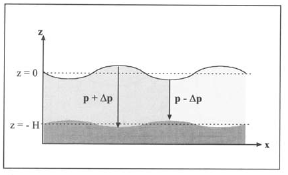
\includegraphics[width=9.0cm]{./img_chap3/img311.png}
      \subcaption{Generating mechanism of the primary microseisms.}\label{img:img311}
    \end{minipage}
    \begin{minipage}[b]{0.65\hsize}
      \centering      
      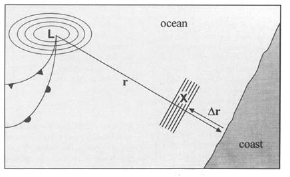
\includegraphics[width=9.0cm]{./img_chap3/img312.png}
      \subcaption{Generating mechanism of the secondary microseisms.}\label{img:img312}
    \end{minipage}
  \end{center}
  \caption{ Generating mechanism of the microsisms. \subref{img:img311} describes the mechanism of the primary microseisms. \subref{img:img312} describes the mechanism of the secondary microseisms.}
\end{figure}


\subsection{Large Earthquakes} \label{sec:313}
hoge\\
...\\
...\\
...\\

Large amplitude earthquakes around the world would interrupt the operation of the gravitational wave detector and reduce their duty cycle. 実際、観測中に地震でロックが落ちたあと、復帰するまでに数時間かかる場合がある \cite{Coughlin2015real}。規模の大きな地震ほど、振幅がおおきいことはもちろん、長周期で減衰までにかかる時間が長い。長周期地震に対して重力波検出器が無力なのは、その防振装置が、せいぜい100 $\mathrm{mHz}$ の地面振動揺れに対して最適化しているためである\cite{}。そのためこのような制御方式を使う以上、制御ノイズが増大して感度が落ちることを犠牲にしてでも、地震が来る前に、地震でロックロスしないような制御フィルターの切り替えを必要とする。この切替のために\textit{Seismon} とよばれる早期地震アラートシステム\cite{Coughlin2017limiting}を用いた制御フィルターの切り替えが試みられている\cite{Biscans2018control}。

hoge\\
...\\
...\\
...\\

\subsection{Air pressure} \label{sec:314}
hoge\\
...\\
...\\
...\\

hoge\\
...\\
...\\
...\\

hoge\\
...\\
...\\
...\\

\subsection{Earth Tides} \label{sec:315}
\cref{sec:311}
hoge\\
...\\
...\\
...\\

hoge\\
...\\
...\\
...\\

hoge\\
...\\
...\\
...\\


\newpage
\section{Long-term Study of the seismic environment at KAGRA}
\subsection{Overview}
The seismic waves are excited on the source and propagate along the surface of the Earth with amplitude decreasing with depth \cite{carter1991high}. However, especially microseims whose peak is around 0.1 $\mathrm{Hz}$ are not attenuated adequately compared with higher frequencies above 1 $\mathrm{Hz}$, because the wavelength is comparable to or longer than the depth. Amount of these atenuation factor is must be explaing by a complicated phenomenon, which depends on either the local geology or location of the exciting sources. 

In this section, seasonal change of the RMS amplitude of the seismic noise is described.

%\cite{naticchioni2014microseismic}。

\subsection{Experimental Arrangement}
Seismic motion is measured by a seismometer installed on the second floor of the X-end area. This area is placed 200 $\mathrm{m}$ underground from the surface of the mountain. Comparison to corner area, human activity in the end area is less because the corner area has parking lots. Comparison to the Y-end area, there is no entrance connected to other mines. Therefore, the X-end area is relatively quiet in the KAGRA mine, regarding the seismic noise induced by human activity.

In this study, Trillium 120-QA which is known as three-component, very broadband, and low-noise seismometer, was used. These three outputs are proportional to the ground velocity of two horizontal and one vertical, respectively. The feature of the low-noise can resolve  Peterson's new low-noise model (NLNM) and new high-noise model (NHNM) \cite{peterson1993observations}.

\begin{figure}[H]
  \begin{center}   
    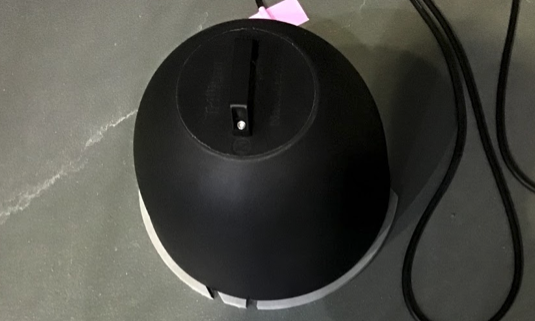
\includegraphics[width=9.0cm]{./img_chap3/img316.png}
    \caption{Trillium 120-QA installed on the second floor at X-end area, which is coverd by black thermal insulation cover}\label{img:img316}
  \end{center}
\end{figure}

As shown in fig \ref{img:img316}, the seismometer is housed in the black thermal insulation cover according to the installation manual \cite{trillium120manual}. Thermal insulation protects two broad categories of thermal couplings that can cause unwanted noise \cite{trillium120manual}. First is the direct coupling to the sensitivity. This coupling typically increases the noise of the vertical channel as a periodic diurnal variation caused by the day-to-night temperature cycle, because the springs that suspended the inertial masses are temperature sensitive. The second is the coupling to tilt from the thermal fluctuation. Tilt converts the vertical acceleration of gravity into horizontal acceleration. This thermally induced tilt noise on the horizontal will be larger than the direct thermal coupling on the vertical channel. To be low sensitivity to both tilt and temperature, this model has a function to center the inertial mass after the initial installation.

The signals of the seismometer is recorded through the data aquisition system developed by LIGO \cite{bork2001overview}. The analog signal is converted to digital signal by the 16 bit analog-to-digital converters (ADC) with 16384 $\mathrm{Hz}$ sampling. In addition, the signal of the seismoemter is amplified with 30 db so that the ADC noise does not mask this signal.\\
...

\subsection{Data}
定常な時系列データを1年間のデータのから選んだ。


\ref{img:img317}.\\
...\\
...\\
\begin{figure}[H]
  \begin{center}   
    
\includegraphics[width=11.0cm]{./img_chap3/img317.png}
    \caption{Available data from June 00 2018 to Jun 00 2019}\label{img:img317}
  \end{center}
\end{figure}

hoge
...\\
...\\
...\\
...\\

hoge
...\\
...\\
...\\
...\\

hoge
...\\
...\\
...\\
...\\

\subsection{Results}
\begin{figure}[h]
  \begin{center}   
    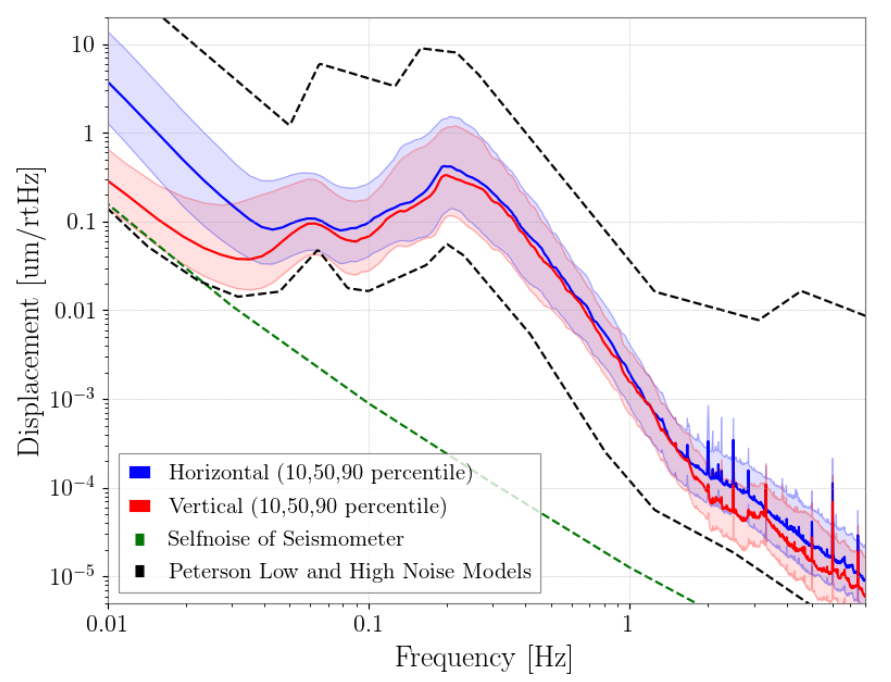
\includegraphics[width=16.0cm]{./img_chap3/img313.png}
    \caption{}\label{img:img317}
  \end{center}
\end{figure}

huge
...\\
...\\
...\\
...\\

\section{Differential Motion Reduction} \label{sec:33}
\subsection{Introduction}
The motion of two mirrors in the cavity have two modes. One is differential motion, which is the length change of that. Another one is common motion, which is the motion of the center of the cavity. In terms of the length control, it is important that the RMS amplitude of differential motion is as small as possible. Actuarlly, the amplitude of these two motions are the same each other when the mirrors moves with no coherence. However, when a coherence exists, the common motion tends to be larger than the differential one. 

As discussed in this section, the coherence depends on both, the arm length and the wavelength of seismic waves. For example, if the arm length is much more smaller than the wavelength, the mirrors move together. This means that the common motion is greater than the differential motion.

The ratio of the amplitudes of the differential motion over common motion is newly defined as Common and Differential Motion Ratio (CDMR). It is usefull to know how the ground reducts the differential motion or increase the common motion. 

\subsection{Differential Motion Reduction}
\subsubsection{Differential Motion and Common Motion}


\begin{figure}[h]
  \begin{center}
    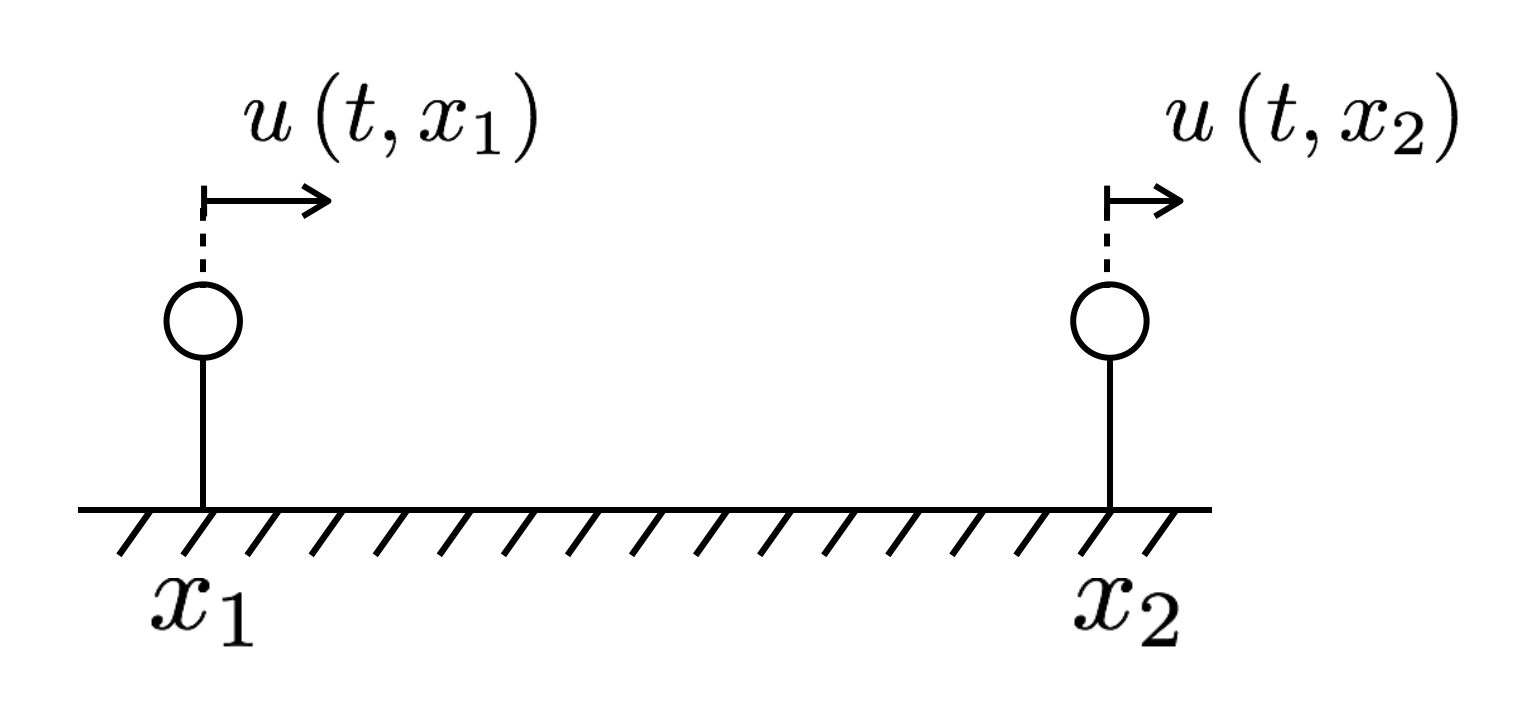
\includegraphics[width=10.0cm]{./img_chap3/img315.png}
    \caption{The displacements of the two points which are sparated L in X axis. }
  \end{center}
\end{figure}


Motions of the two points can be represented as the differential motion and the common motion. Displacement of both differential motion and common motion of the two points shown in Figure(\ref{img:img_chap310}) are defined as
\begin{eqnarray}\label{eq:eq22}
  u_{\mathrm{diff}} \equiv \frac{u_{1}-u_{2}}{\sqrt{2}}, \,
  u_{\mathrm{comm}}  \equiv \frac{u_{1}+u_{2}}{\sqrt{2}}
\end{eqnarray}
where $u_{1}(x,t)$ and $u_2(x,t)$ are the displacement of each points. These two motions defined in Eq.(\ref{eq:eq22}) are normalized by $\sqrt{2}$ due to conserve the total power.


\subsubsection{Common and Differential Motion Ratio (CDMR)}
CDMR is defined as the powers of common motion over the differential motion as bellow,
\begin{equation}
  \mathrm{CDMR} \equiv \sqrt{\frac{\mathrm{Common\,Motion}}{\mathrm{Differential\,Motion}}} = \sqrt{\frac{P_{\mathrm{comm}}(\omega)}{P_{\mathrm{diff}}(\omega)}} \label{eq:eq23}
\end{equation}
where $P_{\mathrm{comm}},P_{\mathrm{diff}}$ are the power spectral densities (PSDs) of the differential motion and common motion, respectively. Each PSDs are converted from the autocorrelation function of these by the Wiener-Khinchin theorem.

First, autocorrelation function $C_{\mathrm{diff}}$ of the differential motion is given by its definition in Eq.(\ref{eq:eq22})
\begin{eqnarray}
  C_{\mathrm{diff}}(\tau) &=& \frac{1}{2}
  \biggl\langle
  \biggl[ x_{1}(t)-x_{2}(t) \biggr] \biggl[ x_{1}(t+\tau)-x_{2}(t+\tau) \biggr]
  \biggr\rangle \\
  &=& \frac{1}{2}\biggl[ C_{11}(\tau) - C_{12}(\tau) - C_{21}(\tau) + C_{22}(\tau) \biggr], 
\end{eqnarray}
,where $C_{ij}$ are the autocorrelation functions of each point and defined as $ C_{ij} \equiv \langle x_{i}(t)x_{j}(t+\tau)\rangle,\, (i=1,2,\,j=1,2)$. Therefore, the power spectrum density of differential motion $P_{\mathrm{diff}}(\omega)$ can be computed as
\begin{eqnarray}
  P_{\mathrm{diff}}(\omega) &=& \frac{1}{2}\biggl[ P_{1}(\omega) + P_{2}(\omega) - P_{12}(\omega) - P_{12}^*(\omega) \biggr]\\
  &=& \frac{1}{2} \biggl[ P_{1}+P_{2} - \mathrm{Re}\left[\gamma \right]\times2\sqrt{P_{1}P_{2}} \biggr] \label{eq:eq31}
\end{eqnarray}
where $P_{1}(\omega),P_{2}(\omega)$ are the power spectrum densities of each points, and $P_{12}(\omega)$ are the cross spectrum between two point. The parameter $\gamma$ is the complex coherence between them defined below,
\begin{eqnarray}
  \gamma \equiv \frac{P_{12}}{\sqrt{P_{1}P_{2}}}.
\end{eqnarray}

Here, assuming that seismic wave propagating each points does not decay, which means $P_{1}=P_{2} \equiv P$, one can compute the $P_{\mathrm{diff}}(\omega)$ as 
\begin{eqnarray}
  P_{\mathrm{diff}}(\omega) = P (1-\mathrm{Re}\left[\gamma\right]).
\end{eqnarray}
Therefore, the PSDs of the common motion can be calculated as
\begin{eqnarray}
  P_{\mathrm{comm}}(\omega) = P (1+\mathrm{Re}\left[\gamma\right]).
\end{eqnarray}
Finaly, CDMR defined Eq.(\ref{eq:eq23}) in case the seismic wave does not decay is represented as
\begin{eqnarray}
 \mathrm{CDMR} = \sqrt{\frac{1 + \mathrm{Re} \left[\gamma \right] }{1 - \mathrm{Re} \left[\gamma \right]}}\,. \label{eq:eq33}
\end{eqnarray}
Eq.(\ref{eq:eq33}) indicate that CDMR can be expressed by only the coherence $\gamma$ between of two points. For example, CDMR tends to be larger when $\gamma$ close to 1. This means that the differential motion is more less than the common motion because the two points move together in the same direction.

\section{Measurement of Differential Motion Reduction}
\subsection{Reduction in X-arm Scale}
\subsection{Reduction in Other Short Scale}



%% \subsubsection{Single Plane Wave Model}
%% The CDMR when single plane wave propagates along the arm cavity is discussed. This model can be applied in the case the source of seismic motion is only one such as an earth quake. Assuming that the plane wave propagates with the azimuth angle $\theta$ along the direction of arm cavity, the wave length $\lambda$ is $\lambda/\mathrm{cos}\theta$. In this situation, the coherence from $x_1$ to $x_2$ is denoted as
%% \begin{equation}
%%   \gamma=e^{i\frac{L\mathrm{cos}\theta\omega}{c}}
%% \end{equation}
%% Therefore, one can compute the CDMR as
%% \begin{equation}  \label{eq:eq18}
%%   \mathrm{CDMR} = \sqrt{\frac{1+\mathrm{cos}(\frac{L\omega}{c}\mathrm{cos}\theta)}{1-\mathrm{cos}(\frac{L\omega}{c}\mathrm{cos}\theta)}}.
%% \end{equation}


%% \subsubsection{Uniform Plane Wave Model}
%% The CDMR when the plane waves are distributed uniformly around the azimuth is discussed. This model can be applied in the case microseisms excite the ground. The coherence is equal to the integral over all direction.
%% \begin{eqnarray} \label{eq:eq19}
%%   \gamma &=& \frac{1}{2\pi} \int_{-\pi}^{\pi} e^{i\frac{\omega}{c} L\cos \theta} d \theta
%% \end{eqnarray}
%% where the coherence is normized azimuth angle. Therefore, the CDMR is given as
%% \begin{equation}  \label{eq:eq20}
%%   \mathrm{CDMR} = \sqrt{\frac{1+J_0(\frac{L\omega}{c})}{1-J_0(\frac{L\omega}{c})}} .
%% \end{equation}





\section{Summary of the Chapter}
